
\documentclass[journal]{IEEEtran}
%
% If IEEEtran.cls has not been installed into the LaTeX system files,
% manually specify the path to it like:
% \documentclass[journal]{../sty/IEEEtran}


\usepackage{hyperref}


% Some very useful LaTeX packages include:
% (uncomment the ones you want to load)


% *** MISC UTILITY PACKAGES ***
%
%\usepackage{ifpdf}
% Heiko Oberdiek's ifpdf.sty is very useful if you need conditional
% compilation based on whether the output is pdf or dvi.
% usage:
% \ifpdf
%   % pdf code
% \else
%   % dvi code
% \fi
% The latest version of ifpdf.sty can be obtained from:
% http://www.ctan.org/tex-archive/macros/latex/contrib/oberdiek/
% Also, note that IEEEtran.cls V1.7 and later provides a builtin
% \ifCLASSINFOpdf conditional that works the same way.
% When switching from latex to pdflatex and vice-versa, the compiler may
% have to be run twice to clear warning/error messages.






% *** CITATION PACKAGES ***
%
\usepackage{cite}
% cite.sty was written by Donald Arseneau
% V1.6 and later of IEEEtran pre-defines the format of the cite.sty package
% \cite{} output to follow that of IEEE. Loading the cite package will
% result in citation numbers being automatically sorted and properly
% "compressed/ranged". e.g., [1], [9], [2], [7], [5], [6] without using
% cite.sty will become [1], [2], [5]--[7], [9] using cite.sty. cite.sty's
% \cite will automatically add leading space, if needed. Use cite.sty's
% noadjust option (cite.sty V3.8 and later) if you want to turn this off.
% cite.sty is already installed on most LaTeX systems. Be sure and use
% version 4.0 (2003-05-27) and later if using hyperref.sty. cite.sty does
% not currently provide for hyperlinked citations.
% The latest version can be obtained at:
% http://www.ctan.org/tex-archive/macros/latex/contrib/cite/
% The documentation is contained in the cite.sty file itself.






% *** GRAPHICS RELATED PACKAGES ***
%
\usepackage[justification=centering]{caption}
\ifCLASSINFOpdf
  \usepackage[pdftex]{graphicx}
  % declare the path(s) where your graphic files are
  % \graphicspath{{../pdf/}{../jpeg/}}
  % and their extensions so you won't have to specify these with
  % every instance of \includegraphics
  % \DeclareGraphicsExtensions{.pdf,.jpeg,.png}
\else
  % or other class option (dvipsone, dvipdf, if not using dvips). graphicx
  % will default to the driver specified in the system graphics.cfg if no
  % driver is specified.
  \usepackage[dvips]{graphicx}
  % declare the path(s) where your graphic files are
  % \graphicspath{{../eps/}}
  % and their extensions so you won't have to specify these with
  % every instance of \includegraphics
  % \DeclareGraphicsExtensions{.eps}
\fi
% graphicx was written by David Carlisle and Sebastian Rahtz. It is
% required if you want graphics, photos, etc. graphicx.sty is already
% installed on most LaTeX systems. The latest version and documentation can
% be obtained at: 
% http://www.ctan.org/tex-archive/macros/latex/required/graphics/
% Another good source of documentation is "Using Imported Graphics in
% LaTeX2e" by Keith Reckdahl which can be found as epslatex.ps or
% epslatex.pdf at: http://www.ctan.org/tex-archive/info/
%
% latex, and pdflatex in dvi mode, support graphics in encapsulated
% postscript (.eps) format. pdflatex in pdf mode supports graphics
% in .pdf, .jpeg, .png and .mps (metapost) formats. Users should ensure
% that all non-photo figures use a vector format (.eps, .pdf, .mps) and
% not a bitmapped formats (.jpeg, .png). IEEE frowns on bitmapped formats
% which can result in "jaggedy"/blurry rendering of lines and letters as
% well as large increases in file sizes.
%
% You can find documentation about the pdfTeX application at:
% http://www.tug.org/applications/pdftex





% *** MATH PACKAGES ***
%
\usepackage{amsmath}
% A popular package from the American Mathematical Society that provides
% many useful and powerful commands for dealing with mathematics. If using
% it, be sure to load this package with the cmex10 option to ensure that
% only type 1 fonts will utilized at all point sizes. Without this option,
% it is possible that some math symbols, particularly those within
% footnotes, will be rendered in bitmap form which will result in a
% document that can not be IEEE Xplore compliant!
%
% Also, note that the amsmath package sets \interdisplaylinepenalty to 10000
% thus preventing page breaks from occurring within multiline equations. Use:
%\interdisplaylinepenalty=2500
% after loading amsmath to restore such page breaks as IEEEtran.cls normally
% does. amsmath.sty is already installed on most LaTeX systems. The latest
% version and documentation can be obtained at:
% http://www.ctan.org/tex-archive/macros/latex/required/amslatex/math/





% *** SPECIALIZED LIST PACKAGES ***
%
%\usepackage{algorithmic}
% algorithmic.sty was written by Peter Williams and Rogerio Brito.
% This package provides an algorithmic environment fo describing algorithms.
% You can use the algorithmic environment in-text or within a figure
% environment to provide for a floating algorithm. Do NOT use the algorithm
% floating environment provided by algorithm.sty (by the same authors) or
% algorithm2e.sty (by Christophe Fiorio) as IEEE does not use dedicated
% algorithm float types and packages that provide these will not provide
% correct IEEE style captions. The latest version and documentation of
% algorithmic.sty can be obtained at:
% http://www.ctan.org/tex-archive/macros/latex/contrib/algorithms/
% There is also a support site at:
% http://algorithms.berlios.de/index.html
% Also of interest may be the (relatively newer and more customizable)
% algorithmicx.sty package by Szasz Janos:
% http://www.ctan.org/tex-archive/macros/latex/contrib/algorithmicx/




% *** ALIGNMENT PACKAGES ***
%
%\usepackage{array}
% Frank Mittelbach's and David Carlisle's array.sty patches and improves
% the standard LaTeX2e array and tabular environments to provide better
% appearance and additional user controls. As the default LaTeX2e table
% generation code is lacking to the point of almost being broken with
% respect to the quality of the end results, all users are strongly
% advised to use an enhanced (at the very least that provided by array.sty)
% set of table tools. array.sty is already installed on most systems. The
% latest version and documentation can be obtained at:
% http://www.ctan.org/tex-archive/macros/latex/required/tools/


%\usepackage{mdwmath}
%\usepackage{mdwtab}
% Also highly recommended is Mark Wooding's extremely powerful MDW tools,
% especially mdwmath.sty and mdwtab.sty which are used to format equations
% and tables, respectively. The MDWtools set is already installed on most
% LaTeX systems. The lastest version and documentation is available at:
% http://www.ctan.org/tex-archive/macros/latex/contrib/mdwtools/


% IEEEtran contains the IEEEeqnarray family of commands that can be used to
% generate multiline equations as well as matrices, tables, etc., of high
% quality.


%\usepackage{eqparbox}
% Also of notable interest is Scott Pakin's eqparbox package for creating
% (automatically sized) equal width boxes - aka "natural width parboxes".
% Available at:
% http://www.ctan.org/tex-archive/macros/latex/contrib/eqparbox/





% *** SUBFIGURE PACKAGES ***
%\usepackage[tight,footnotesize]{subfigure}
% subfigure.sty was written by Steven Douglas Cochran. This package makes it
% easy to put subfigures in your figures. e.g., "Figure 1a and 1b". For IEEE
% work, it is a good idea to load it with the tight package option to reduce
% the amount of white space around the subfigures. subfigure.sty is already
% installed on most LaTeX systems. The latest version and documentation can
% be obtained at:
% http://www.ctan.org/tex-archive/obsolete/macros/latex/contrib/subfigure/
% subfigure.sty has been superceeded by subfig.sty.



%\usepackage[caption=false]{caption}
%\usepackage[font=footnotesize]{subfig}
% subfig.sty, also written by Steven Douglas Cochran, is the modern
% replacement for subfigure.sty. However, subfig.sty requires and
% automatically loads Axel Sommerfeldt's caption.sty which will override
% IEEEtran.cls handling of captions and this will result in nonIEEE style
% figure/table captions. To prevent this problem, be sure and preload
% caption.sty with its "caption=false" package option. This is will preserve
% IEEEtran.cls handing of captions. Version 1.3 (2005/06/28) and later 
% (recommended due to many improvements over 1.2) of subfig.sty supports
% the caption=false option directly:
%\usepackage[caption=false,font=footnotesize]{subfig}
%
% The latest version and documentation can be obtained at:
% http://www.ctan.org/tex-archive/macros/latex/contrib/subfig/
% The latest version and documentation of caption.sty can be obtained at:
% http://www.ctan.org/tex-archive/macros/latex/contrib/caption/




% *** FLOAT PACKAGES ***
%
%\usepackage{fixltx2e}
% fixltx2e, the successor to the earlier fix2col.sty, was written by
% Frank Mittelbach and David Carlisle. This package corrects a few problems
% in the LaTeX2e kernel, the most notable of which is that in current
% LaTeX2e releases, the ordering of single and double column floats is not
% guaranteed to be preserved. Thus, an unpatched LaTeX2e can allow a
% single column figure to be placed prior to an earlier double column
% figure. The latest version and documentation can be found at:
% http://www.ctan.org/tex-archive/macros/latex/base/



%\usepackage{stfloats}
% stfloats.sty was written by Sigitas Tolusis. This package gives LaTeX2e
% the ability to do double column floats at the bottom of the page as well
% as the top. (e.g., "\begin{figure*}[!b]" is not normally possible in
% LaTeX2e). It also provides a command:
%\fnbelowfloat
% to enable the placement of footnotes below bottom floats (the standard
% LaTeX2e kernel puts them above bottom floats). This is an invasive package
% which rewrites many portions of the LaTeX2e float routines. It may not work
% with other packages that modify the LaTeX2e float routines. The latest
% version and documentation can be obtained at:
% http://www.ctan.org/tex-archive/macros/latex/contrib/sttools/
% Documentation is contained in the stfloats.sty comments as well as in the
% presfull.pdf file. Do not use the stfloats baselinefloat ability as IEEE
% does not allow \baselineskip to stretch. Authors submitting work to the
% IEEE should note that IEEE rarely uses double column equations and
% that authors should try to avoid such use. Do not be tempted to use the
% cuted.sty or midfloat.sty packages (also by Sigitas Tolusis) as IEEE does
% not format its papers in such ways.


%\ifCLASSOPTIONcaptionsoff
%  \usepackage[nomarkers]{endfloat}
% \let\MYoriglatexcaption\caption
% \renewcommand{\caption}[2][\relax]{\MYoriglatexcaption[#2]{#2}}
%\fi
% endfloat.sty was written by James Darrell McCauley and Jeff Goldberg.
% This package may be useful when used in conjunction with IEEEtran.cls'
% captionsoff option. Some IEEE journals/societies require that submissions
% have lists of figures/tables at the end of the paper and that
% figures/tables without any captions are placed on a page by themselves at
% the end of the document. If needed, the draftcls IEEEtran class option or
% \CLASSINPUTbaselinestretch interface can be used to increase the line
% spacing as well. Be sure and use the nomarkers option of endfloat to
% prevent endfloat from "marking" where the figures would have been placed
% in the text. The two hack lines of code above are a slight modification of
% that suggested by in the endfloat docs (section 8.3.1) to ensure that
% the full captions always appear in the list of figures/tables - even if
% the user used the short optional argument of \caption[]{}.
% IEEE papers do not typically make use of \caption[]'s optional argument,
% so this should not be an issue. A similar trick can be used to disable
% captions of packages such as subfig.sty that lack options to turn off
% the subcaptions:
% For subfig.sty:
% \let\MYorigsubfloat\subfloat
% \renewcommand{\subfloat}[2][\relax]{\MYorigsubfloat[]{#2}}
% For subfigure.sty:
% \let\MYorigsubfigure\subfigure
% \renewcommand{\subfigure}[2][\relax]{\MYorigsubfigure[]{#2}}
% However, the above trick will not work if both optional arguments of
% the \subfloat/subfig command are used. Furthermore, there needs to be a
% description of each subfigure *somewhere* and endfloat does not add
% subfigure captions to its list of figures. Thus, the best approach is to
% avoid the use of subfigure captions (many IEEE journals avoid them anyway)
% and instead reference/explain all the subfigures within the main caption.
% The latest version of endfloat.sty and its documentation can obtained at:
% http://www.ctan.org/tex-archive/macros/latex/contrib/endfloat/
%
% The IEEEtran \ifCLASSOPTIONcaptionsoff conditional can also be used
% later in the document, say, to conditionally put the References on a 
% page by themselves.





% *** PDF, URL AND HYPERLINK PACKAGES ***
%
%\usepackage{url}
% url.sty was written by Donald Arseneau. It provides better support for
% handling and breaking URLs. url.sty is already installed on most LaTeX
% systems. The latest version can be obtained at:
% http://www.ctan.org/tex-archive/macros/latex/contrib/misc/
% Read the url.sty source comments for usage information. Basically,
% \url{my_url_here}.





% *** Do not adjust lengths that control margins, column widths, etc. ***
% *** Do not use packages that alter fonts (such as pslatex).         ***
% There should be no need to do such things with IEEEtran.cls V1.6 and later.
% (Unless specifically asked to do so by the journal or conference you plan
% to submit to, of course. )


% correct bad hyphenation here
\hyphenation{op-tical net-works semi-conduc-tor}


\begin{document}

\title{Sequence Based T~Cell Epitope Prediction: Verification and Iprovements}

\author{Alexander~Crowell,~Jack~Holland,~and~Vineetha~Paruchuri}


% make the title area
\maketitle


\begin{abstract}
%\boldmath
Successful prediction of T~cell epitopes is very useful in vaccine design and immunotherapy. Obviously, computational prediction is a lot cheaper than experimental validation for T~cell epitope prediction. Researchers have previously predicted T~cell epitopes in both a pan specific and allele specific fashion with varying degrees of success. In this paper, we apply machine learning, specifically Support Vector Machines, to predict T~cell epitopes, and compare our results to the leading approaches: NetMHCII, NetMHCIIpan, and the MultiRTA methods. Our analysis showed that <insert data> 
\end{abstract}


% Note that keywords are not normally used for peerreview papers.
\begin{IEEEkeywords}
T~Cell Epitopes, Epitope Mapping, Epitope Prediction, NetMHC, MultiRTA, Neural Networks, Support Vector Machines, Machine Learning.
\end{IEEEkeywords}





\section{Introduction}

\IEEEPARstart{T}{cell} epitopes are the part of an antigen, usually a specific peptide sequence, which is bound by the Major Histocompatibility Complex (MHC). There are two types of MHC proteins, MHC I, which is present on all cells, and MHC II, which is only present on antigen-presenting cells. Due to differences in the structure of their binding pockets, T~cell peptides bound by MHC class I molecules are between 8 and 11 amino acids in length, whereas those presented by MHC class II are 13-17 amino acids in length. 

The high degree of polymorphism exhibited by MHC II alleles means that experimental validation of epitope regions is cost intensive. Hence, the computational methods for accurate prediction of binding peptides to class II molecules is a topic of interest. Researchers have previously tried to computationally predict T~cell epitopes, with various degrees of success, using Artificial Neural Networks, such as in NetMHCII \cite{NetMHCII} and NetMHCIIpan \cite{NetMHCIIpan}, or Position Specific Scoring Matrix such as in TEPITOPEpan \cite{TEPITOPEpan}, or Position Weight Matrix, such as in PREDIVAC \cite{PREDIVAC}. 

In this project, we use the machine learning technique of Support Vector Machines to predict T~cell epitopes, and compare the performance of our approach to allele-specific and pan-specific approaches like NetMHC, NetMHCIIpan, TEPITOPE \cite{TEPITOPE}, and MultiRTA \cite{MultiRTA}. The results show that <insert something about our performance>


\section{NetMHCII}
NetMHCII is a neural network based approach for MHC class II predictions. It uses a novel artificial neural network-based method, \textit{NN-align}, which allows for simultaneous identification of the MHC class II binding core and binding affinity. As mentioned in \cite{NetMHCII}, the NN-align method includes ``explicit encoding of the peptide flanking residues in terms of amino acid composition and length, as well as a novel scheme for neural network training that deals with the data redundancy inherent in the peptide data due to multiple examples of identical binding cores". The NN-align method is trained on a large data set of more than 14,000 quantitative peptide MHC binding values covering 14 HLA-DR alleles.

\subsection{NetMHCII Implementation}
The implementation of NN-align was done as an artificial neural network. It was done as a two-step procedure that simultaneously estimated the optimal peptide binding register, and the network weight configuration (where the network weights were updated using gradient descent back propogation). The score of a 9 mer peptide was calculated using the conventional feed-forward algorithm. The incorporation of information from residues flanking the peptide binding core seemed to considerably improve the predictive performance of the method. 

%\begin{figure}[!t]
%\centering
%\includegraphics[width=2.5in]{myfigure}
% where an .eps filename suffix will be assumed under latex, 
% and a .pdf suffix will be assumed for pdflatex; or what has been declared
% via \DeclareGraphicsExtensions.
%\caption{Simulation Results}
%\label{fig_sim}
%\end{figure}


\subsection{NetMHCII Performance, and Metrics Used}
In NetMHCII, all statistical comparisons were made using one-tailed binomial tests. For each comparison, it was calculated how often one method outperforms the other (excluding ties). One-tailed p-values were calculated based on these numbers. P-values < 0.05 were taken to be significant. Performance across different methods was calculated using AUC.

\subsection{NetMHCII in Context}
NetMHCII provided both a new perspective on and one of the best examples of the application of machine learning to T~cell epitope prediction.  As a result it was a natural choice as a comparison point for our study.  Since SVMs and Neural Networks are such distinct approaches we also hoped that our approach might capture some independent insight.


\section{Support Vector Machines}
Support Vector Machine is a supervised learning algorithm used for classification and regression analysis - they identify patterns in the data. Once we train the SVM on some data (called the training data set), it classifies new examples into one of two classes, thereby making it a non-probablistic binary linear classifier. An SVM can also perform non-linear classification using \textit{kernel trick}, which just means that it doesn't need to compute the coordinates of data in a high-dimensional space, but rather just the inner products between images of all pairs of data, thereby making it computationally cheaper. 

Given the fact that it is a binary linear classifier that also performs non-linear classification, we felt that, as a first step, using SVM as the choice of machine learning algorithm made sense. 

\subsection{Formal Definition}

From Wikipedia,\\ 
Given some training data $D$, a set of $n$ points of the form 

$$
D =   \lbrace \left(x_{i}, y_{i}\right) \mid x_{i} \in R^{p}, y_{i} \in \lbrace-1, 1\rbrace\rbrace_{i=1}^n     
$$
    
where the $y_i$ is either 1 or −1, indicating the class to which the point $x_i$ belongs. Each $x_i$ is a p-dimensional real vector. We want to find the maximum-margin hyperplane that divides the points having $y_i=1$ from those having $y_i=-1$. Any hyperplane can be written as the set of points $x$ satisfying 

$$
\mathbf{w}.x - b = 0,
$$
where $\cdot$ denotes the dot product and $w$ the (not necessarily normalized) normal vector to the hyperplane. The parameter $\tfrac{b}{\|\mathbf{w}\|}$ determines the offset of the hyperplane from the origin along the normal vector ${\mathbf{w}}$.\\

If the training data is linearly separable, we can separate the examples under two hyperplanes such that there are no points between them. We can then try to maximize their distance. The region bound by these hyperplanes is called "the margin", and ideally, we want to maximize it so that there is no overlap.

These hyperplanes can be described by the equations


$$
    \mathbf{w}.\mathbf{x} - b = 1    \quad \textrm{and} \quad 
    \mathbf{w}.\mathbf{x} - b = -1
$$

We then find the geometric distance between these two hyperplanes is $\tfrac{2}{\|\mathbf{w}\|}$, so we want to minimize $\|\mathbf{w}\|$. We also add the below constraint because we want to prevent the data points from falling under the margin:\\ 

For each $i$ either
$$\mathbf{w}\cdot\mathbf{x}_i - b \ge 1\qquad\text{ for }\mathbf{x}_i$$ 
of the first class, or
$$\mathbf{w}\cdot\mathbf{x}_i - b \le -1\qquad\text{ for }\mathbf{x}_i$$ 
of the second.  \\  

Which can be written as:
$$
    y_i(\mathbf{w}\cdot\mathbf{x}_i - b) \ge 1, \quad \text{ for all } 1 \le i \le n.\qquad\qquad(1)
$$

We can express the above as an optimization problem:

Minimize $(in \quad {\mathbf{w},b})$
$$   
 \|\mathbf{w}\|
$$
 
subject to $(for \enskip any \enskip i = 1, \dots, n)$
$$
y_i(\mathbf{w}\cdot\mathbf{x_i} - b) \ge 1. \,
$$

The optimization problem presented above can be converted into a quadratic programming optimization problem, which gives the primal and dual forms of the SVM. In this project, we used the dual form of the SVM, ``which reveals that the maximum-margin hyperplane, and therefore the classification task is only a function of the support vectors" \cite{WikipediaSVM}.


\section{Methods}
This section provides a brief overview of how we implemented our algorithm and how we validated it.

\subsection{Datasets}
We took the peptides from IEDB, and subdivided them according to allele type. We also tried out other data repositories, like the Dana-Farber \cite{DanaFarber} repository, but since all entries in it have a positive binding value, we didn't find it suitable for our problem. We also ran our algorithm on the MultiRTA \cite{MultiRTA} dataset. Data selection and sanitization is a crucial step here, because any irregularities in data can affect the learning of the SVM in unpredictable ways.

\subsection{Implementation of the SVM and Metrics}
We implemented SVM in python using scikit-learn \cite{ScikitLearn}, and used scikit-learn functions such as \textit{roc\_auc\_score} etc. for metrics.

\subsection{Encoding Peptides}
Peptides were encoded using the built in multilabel binarizer included in scikit learn preprocessing library.  Initially each amino acid is mapped to an integer.  The resulting lists of integers are then passed to the multilabel binarizer, producing a binarized list which can be passed to the SVM.


\subsection{AUC as a Comparison Metric} 
\textit{Area Under the Curve (AUC)} is used as a metric throughout, because other approaches used the same metric or comparable metrics. Also, some of our data is skewed, and since AUC accounts for both true and false positives, it ensures that any good predictions we get isn't due to the fact that we have more positives in our data.


\section{Results}

\subsection{Individual Alleles}
Results across alleles for the allele specific methods are relatively consistent with the exception of HLA-DRA*01:01 for which more data exists than the other alleles.  SMM-align and the neural net based methods show considerable relative improvement for this allele suggesting they are gaining more information from the increased amount of data.

\begin{figure}[!t]
\centering
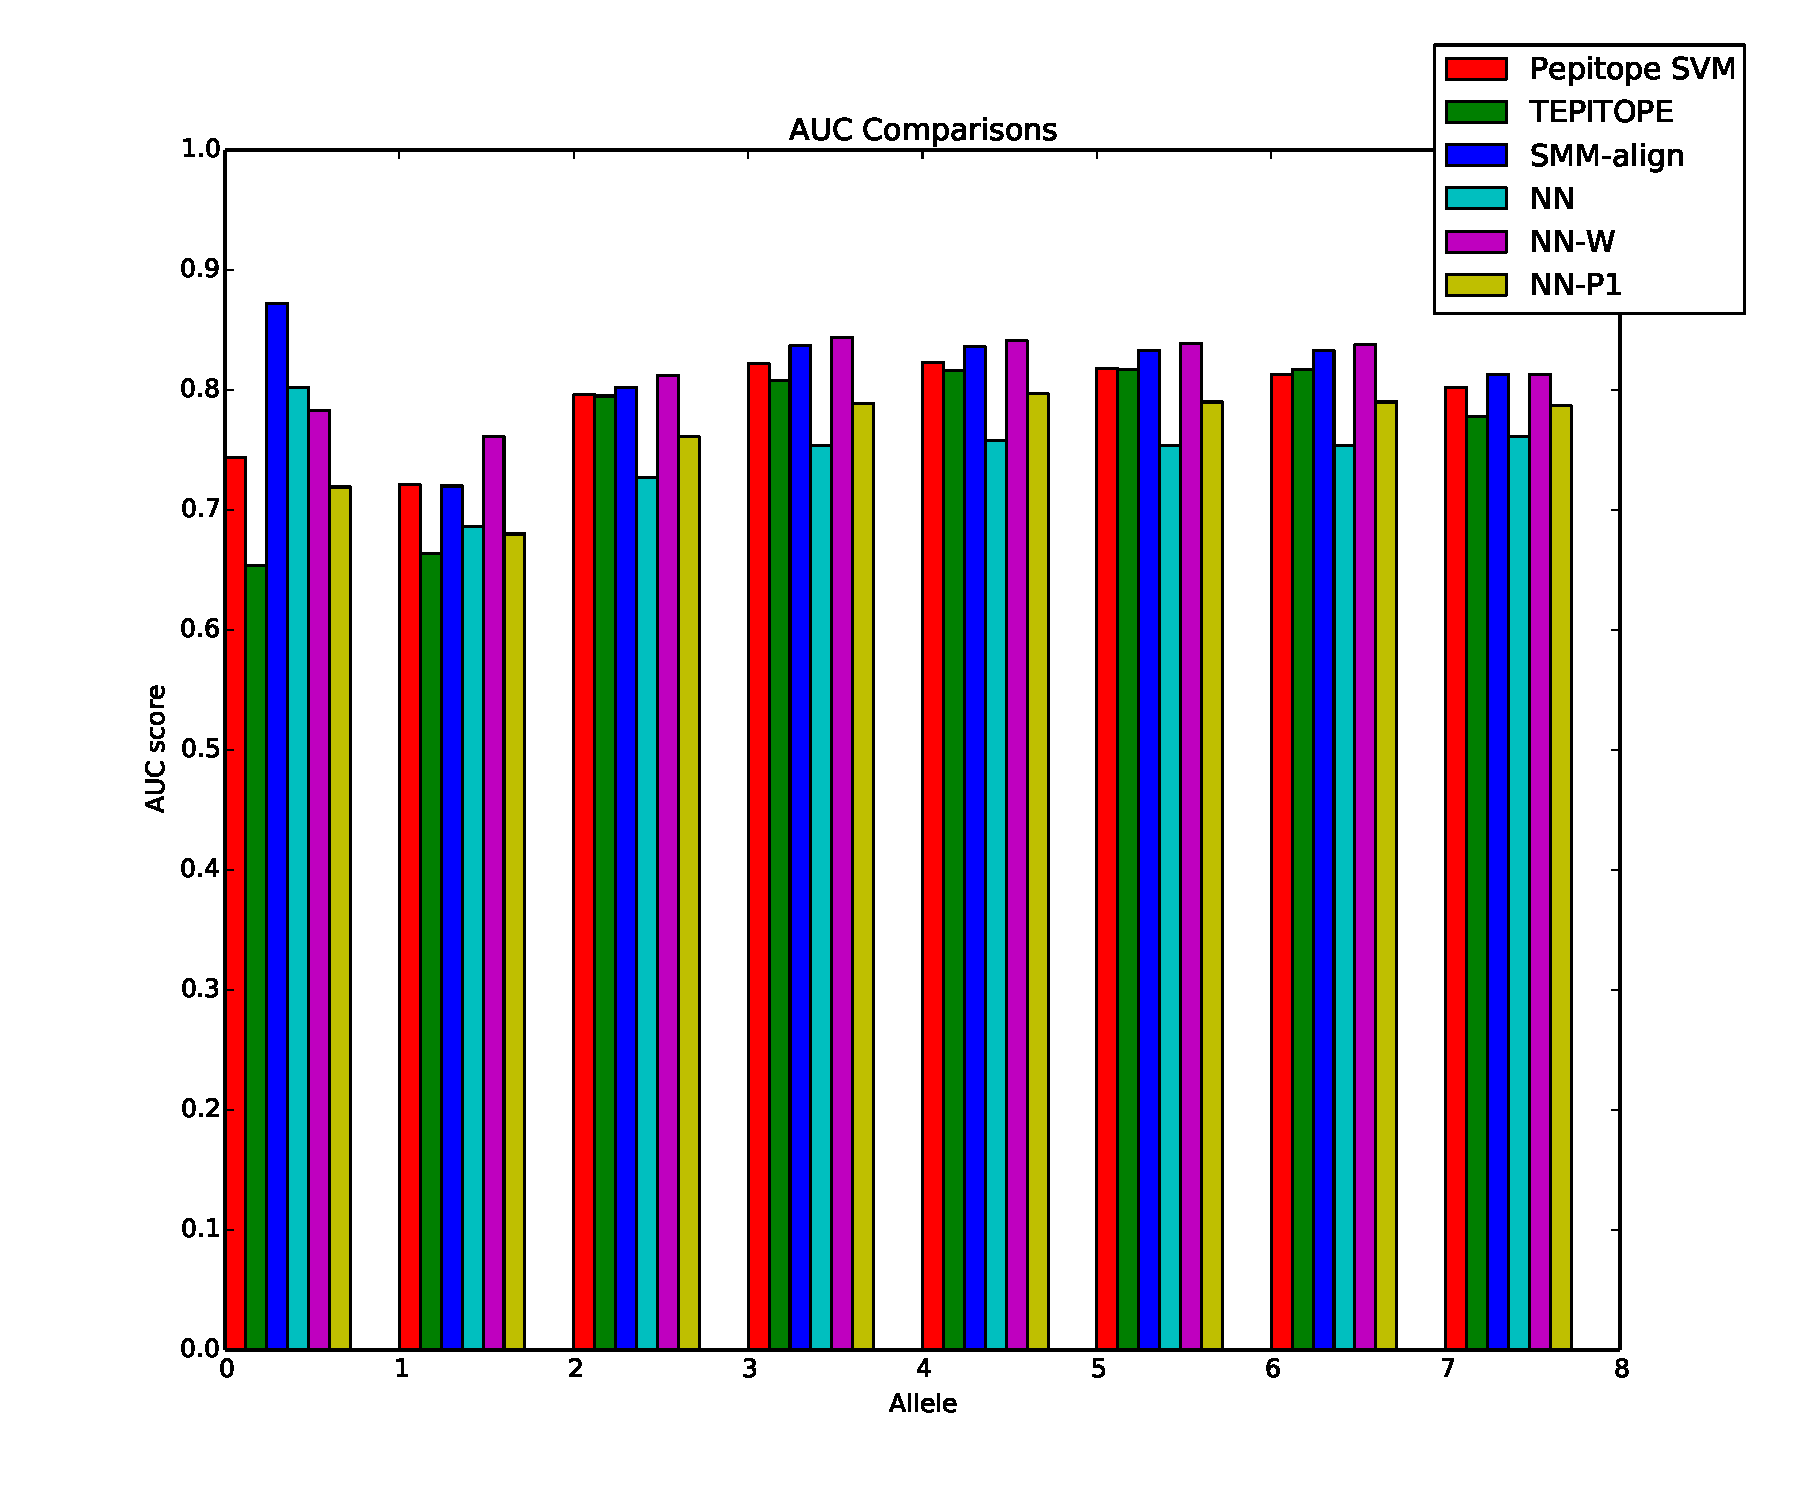
\includegraphics[width=2.5in]{individual}
\caption{AUC as a Function of Prediction Method and Allele}
\label{fig_sim}
\end{figure}


\subsection{Combined Alleles}
Pooled results for each of the allele-specific methods suggest the superiority of neural net based approaches with intermediate success being achieved by our method and SMM-align and Tepitope providing the worst results.
\begin{figure}[!t]
\centering
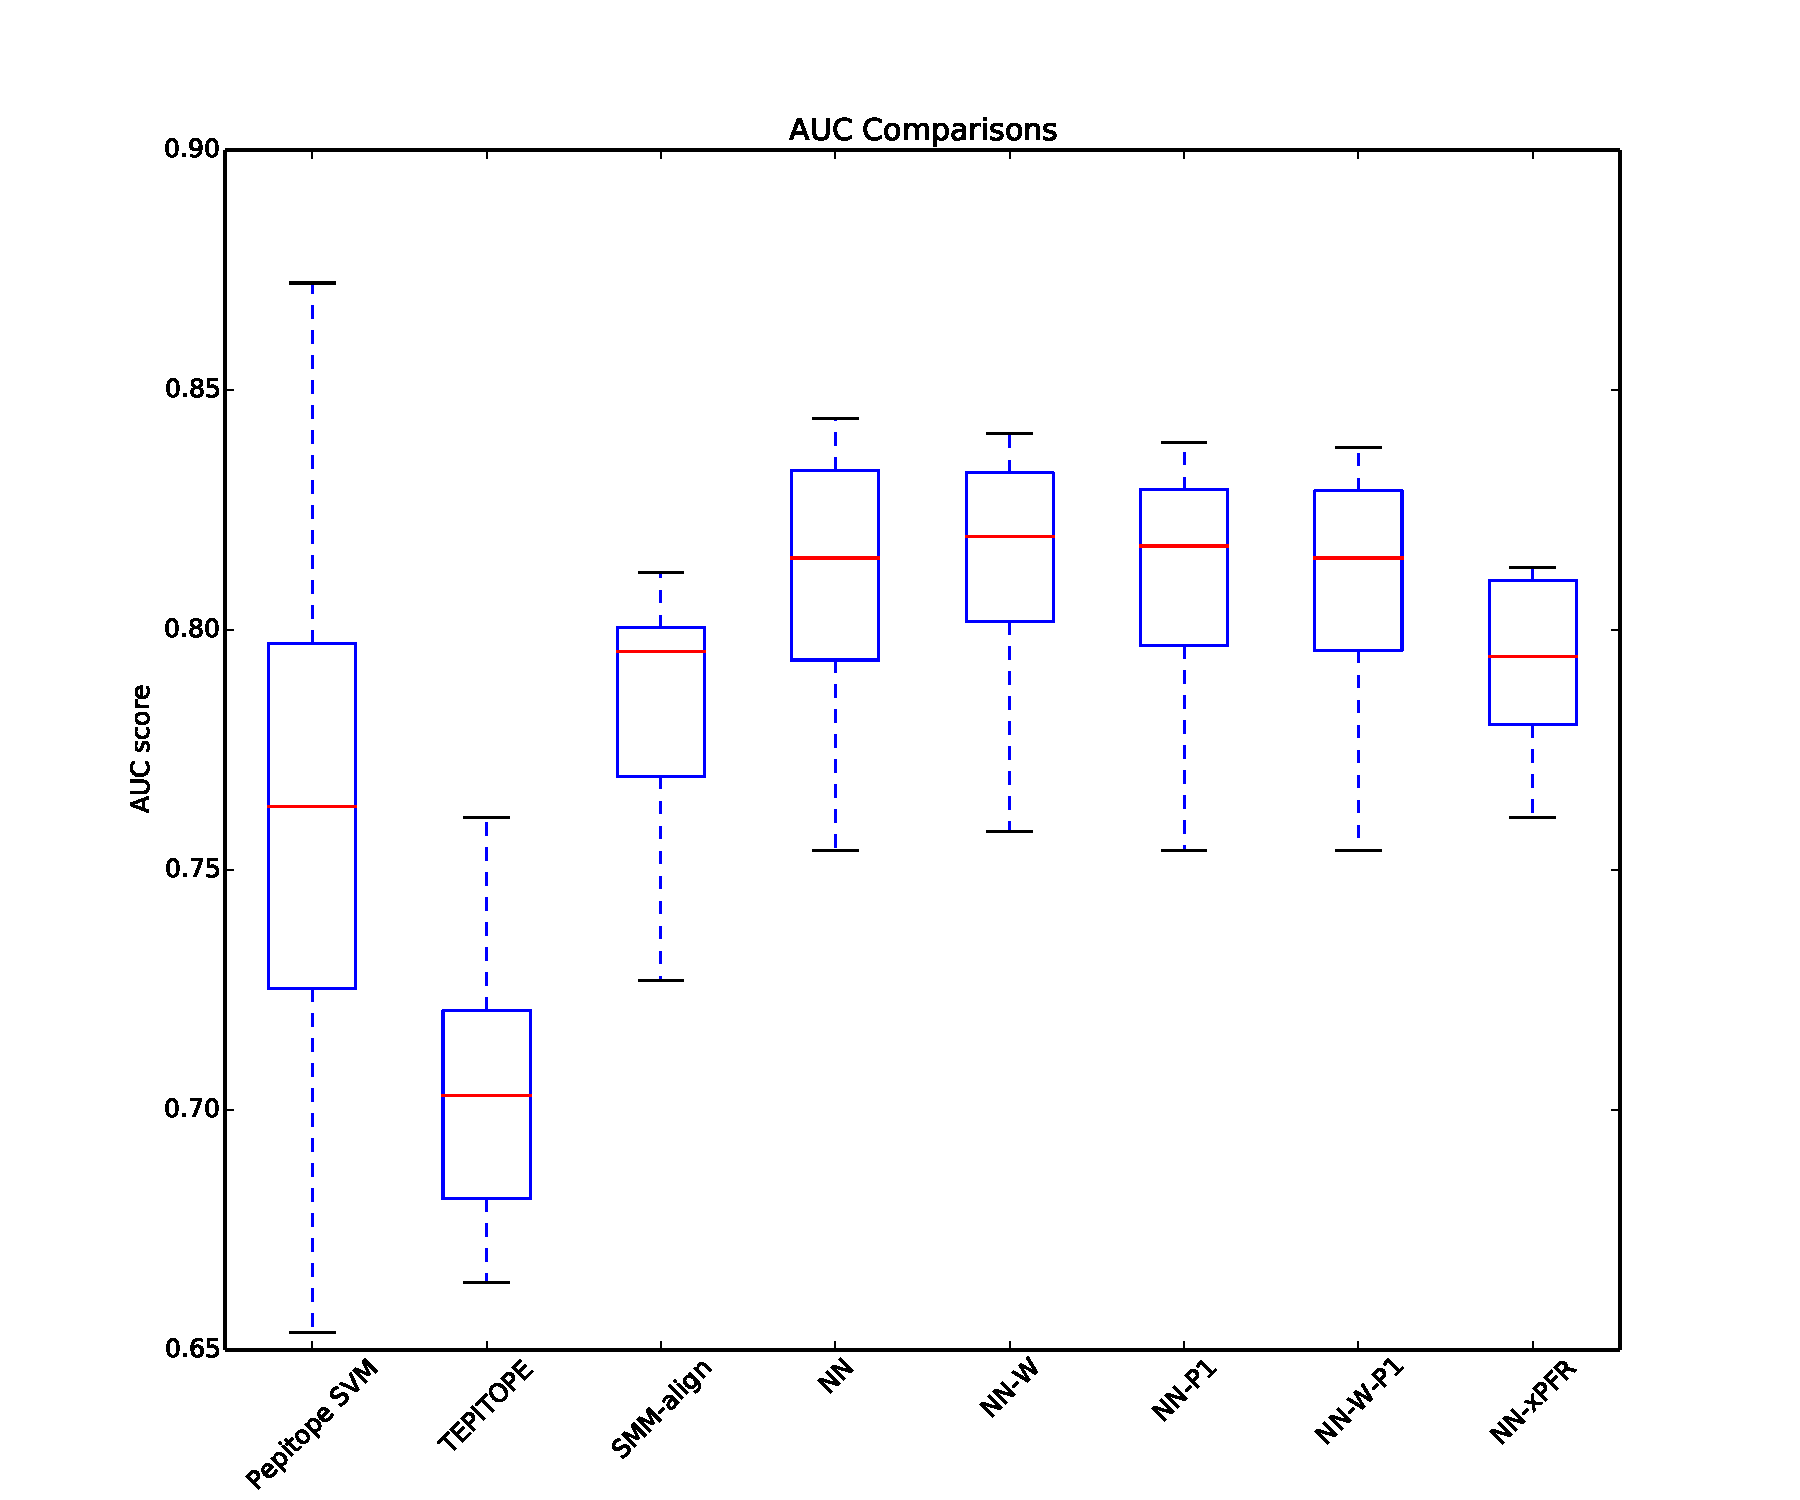
\includegraphics[width=2.5in]{combined}
\caption{AUC as a Function of Prediction Method}
\label{fig_sim}
\end{figure}


\subsection{Results Compared to MultiRTA}
\subsection{Results Compared to NetMHCII}
\subsection{Results Compared to NetMHCIIpan}
Can describe what results we got in cross validaton, what we compared to, how it scaled up etc.

Also figures ``iterations.pdf" and ``skew\_v\_auc" are just floating around so once we put in text I'll look for optimal placement of those. For now just including the code. 

\begin{figure}[!h]
\centering
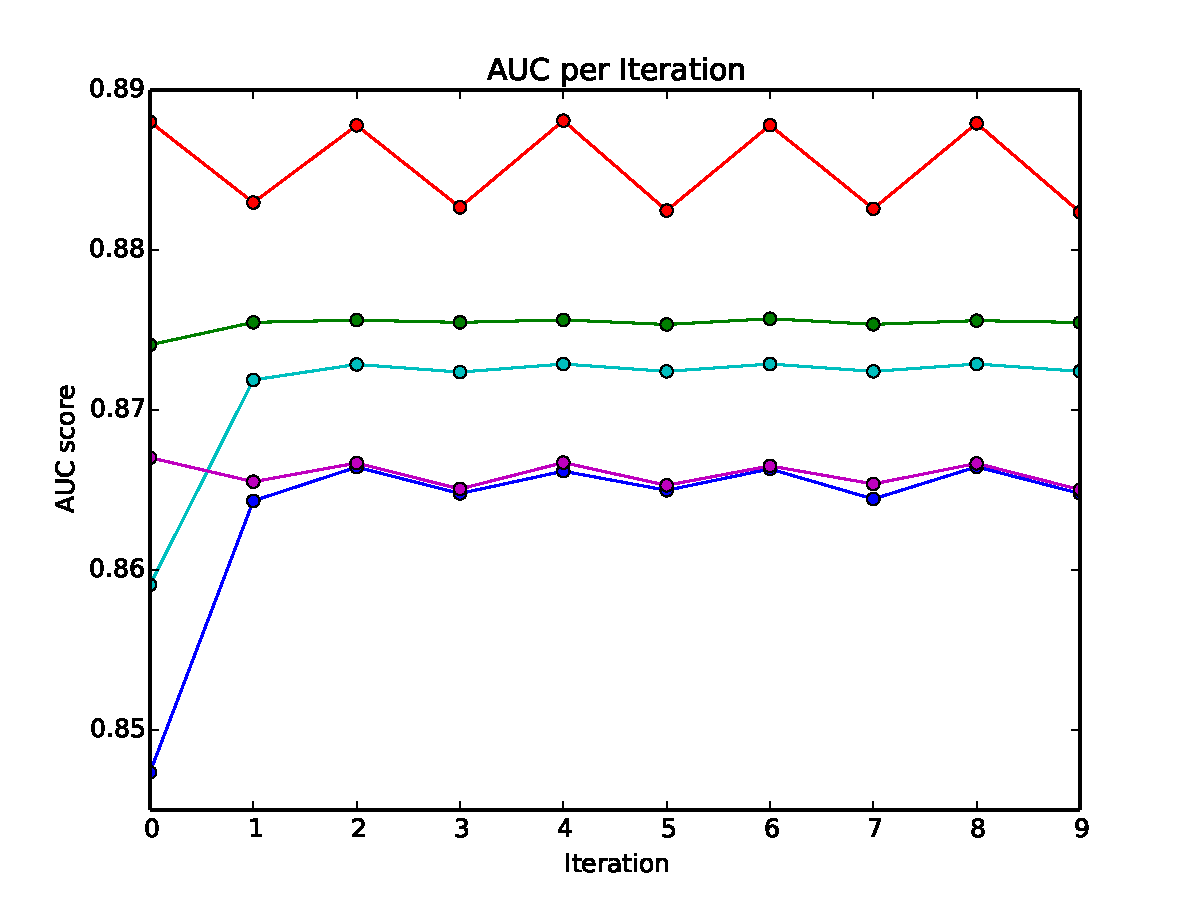
\includegraphics[width=3.8in]{iterations}
\caption{Nonamer Selection: AUC as a Function of Iteration}
\label{fig_sim}
\end{figure}

\begin{figure}[!h]
\centering
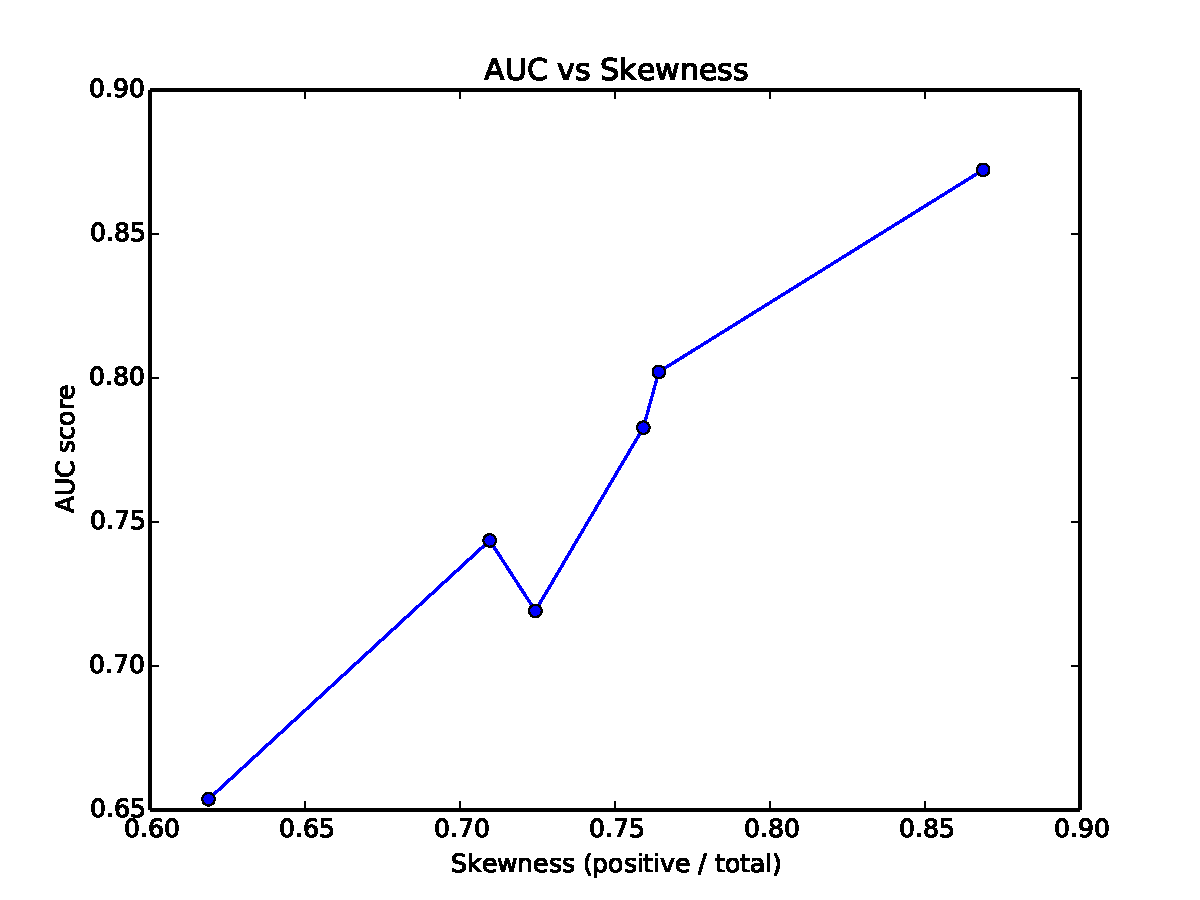
\includegraphics[width=3.8in]{skew_v_auc}
\caption{Ratio of Binding and Non-Binding Peptides vs AUC}
\label{fig_sim}
\end{figure}



\section{Conclusion}
There were no significant differences - assuming a normal distribution - between our method and any of the others.  This result was clearly due to the breadth of our results distribution.  When simply considering the means, our method  performed similarly to SMM-align, and was superior to Tepitope but inferior to NetMHCII.  It is important to observe that for our binary classifier based method, we employed qualitative binding data directly from the IEDB rather than the published NetMHCII and MultiRTA datasets.  We performed a parameter search of kd thresholds for the NetMHCII and MultiRTA datasets but found that the AUC was heavily influenced by the degree of uneveness in the data distribution.  Similarly, when we plotted AUC for each allele against the ratio of binding to non-binding peptides, we found a strong correlation.  These two results in combination raised some concern on our part not only for the validity of our predictions but also for what portion of the other methods effectiviness was simply a result of the data's distribution.  Overall our method did not improve on the state of the art.  Our analysis does suggest however that the AUC absent any information about the data distribution is not informative and that consequently, unevenly distributed data may be more problematic than previously appreciated.





% if have a single appendix:
%\appendix[Proof of the Zonklar Equations]
% or
%\appendix  % for no appendix heading
% do not use \section anymore after \appendix, only \section*
% is possibly needed

% use appendices with more than one appendix
% then use \section to start each appendix
% you must declare a \section before using any
% \subsection or using \label (\appendices by itself
% starts a section numbered zero.)
%

% An example of a floating figure using the graphicx package.
% Note that \label must occur AFTER (or within) \caption.
% For figures, \caption should occur after the \includegraphics.
% Note that IEEEtran v1.7 and later has special internal code that
% is designed to preserve the operation of \label within \caption
% even when the captionsoff option is in effect. However, because
% of issues like this, it may be the safest practice to put all your
% \label just after \caption rather than within \caption{}.
%
% Reminder: the "draftcls" or "draftclsnofoot", not "draft", class
% option should be used if it is desired that the figures are to be
% displayed while in draft mode.
%
%\begin{figure}[!t]
%\centering
%\includegraphics[width=2.5in]{myfigure}
% where an .eps filename suffix will be assumed under latex, 
% and a .pdf suffix will be assumed for pdflatex; or what has been declared
% via \DeclareGraphicsExtensions.
%\caption{Simulation Results}
%\label{fig_sim}
%\end{figure}

% Note that IEEE typically puts floats only at the top, even when this
% results in a large percentage of a column being occupied by floats.


% An example of a double column floating figure using two subfigures.
% (The subfig.sty package must be loaded for this to work.)
% The subfigure \label commands are set within each subfloat command, the
% \label for the overall figure must come after \caption.
% \hfil must be used as a separator to get equal spacing.
% The subfigure.sty package works much the same way, except \subfigure is
% used instead of \subfloat.
%
%\begin{figure*}[!t]
%\centerline{\subfloat[Case I]\includegraphics[width=2.5in]{subfigcase1}%
%\label{fig_first_case}}
%\hfil
%\subfloat[Case II]{\includegraphics[width=2.5in]{subfigcase2}%
%\label{fig_second_case}}}
%\caption{Simulation results}
%\label{fig_sim}
%\end{figure*}
%
% Note that often IEEE papers with subfigures do not employ subfigure
% captions (using the optional argument to \subfloat), but instead will
% reference/describe all of them (a), (b), etc., within the main caption.


% An example of a floating table. Note that, for IEEE style tables, the 
% \caption command should come BEFORE the table. Table text will default to
% \footnotesize as IEEE normally uses this smaller font for tables.
% The \label must come after \caption as always.
%
%\begin{table}[!t]
%% increase table row spacing, adjust to taste
%\renewcommand{\arraystretch}{1.3}
% if using array.sty, it might be a good idea to tweak the value of
% \extrarowheight as needed to properly center the text within the cells
%\caption{An Example of a Table}
%\label{table_example}
%\centering
%% Some packages, such as MDW tools, offer better commands for making tables
%% than the plain LaTeX2e tabular which is used here.
%\begin{tabular}{|c||c|}
%\hline
%One & Two\\
%\hline
%Three & Four\\
%\hline
%\end{tabular}
%\end{table}




\appendices
\section{Division of Work}
\subsection{Alexander Crowell}
\subsection{Jack Holland}
\subsection{Vineetha Paruchuri}

%% you can choose not to have a title for an appendix
%% if you want by leaving the argument blank
%\section{}
%Appendix two text goes here.


% use section* for acknowledgement
%\section*{Acknowledgment}
%
%
%The authors would like to thank...
%
%
%% Can use something like this to put references on a page
%% by themselves when using endfloat and the captionsoff option.
%\ifCLASSOPTIONcaptionsoff
%  \newpage
%\fi



% trigger a \newpage just before the given reference
% number - used to balance the columns on the last page
% adjust value as needed - may need to be readjusted if
% the document is modified later
%\IEEEtriggeratref{8}
% The "triggered" command can be changed if desired:
%\IEEEtriggercmd{\enlargethispage{-5in}}

% references section


\begin{thebibliography}{1}

%\bibitem{IEEEhowto:kopka}
%H.~Kopka and P.~W. Daly, \emph{A Guide to \LaTeX}, 3rd~ed.\hskip 1em plus
%  0.5em minus 0.4em\relax Harlow, England: Addison-Wesley, 1999.
  


\bibitem{NetMHCII}
Nielsen~M, Lund~O, \emph{NN-align. An artificial neural network-based alignment algorithm for MHC class II peptide binding prediction}, \hskip 1em plus
  0.5em minus 0.4em\relax In proc. BMC Bioinformatics. 2009.
  
\bibitem{NetMHCIIpan}
Nielsen~M, Lundegaard~C, Blicher~T, Peters~B, Sette~A, Justesen~S, Buus~S, Lund~O, \emph{Quantitative predictions of peptide binding to any HLA-DR molecule of known sequence: NetMHCIIpan}, \hskip 1em plus
  0.5em minus 0.4em\relax PLoS Comput Biol. 2008.
  
  
\bibitem{TEPITOPEpan}
Zhang~L, Chen~Y, Wong~H-S, Zhou~S, Mamitsuka~H, et~al., \emph{TEPITOPEpan: Extending TEPITOPE for Peptide Binding Prediction Covering over 700 HLA-DR Molecules}, \hskip 1em plus
  0.5em minus 0.4em\relax PLoS ONE 7(2): e30483, 2012.
  
\bibitem{PREDIVAC}
Oyarz\'{u}n, Patricio, et~al. \emph{PREDIVAC: CD4+ T-cell epitope prediction for vaccine design that covers 95\% of HLA class II DR protein diversity}, \hskip 1em plus
  0.5em minus 0.4em\relax In proc. BMC bioinformatics 14.1, 2013, pp.52.

\bibitem{TEPITOPE}
Sturniolo~T, Bono~E, Ding~J, Raddrizzani~L, Tuereci~O, et~al, \emph{Generation of tissue-specific and promiscuous HLA ligand database using DNA microarrays and virtual HLA class II matrices}, 17th~ed \hskip 1em plus
  0.5em minus 0.4em\relax Nat Biotechnol., 1999, pp.555\textendash561. 

\bibitem{MultiRTA}
Bordner~AJ, Mittelmann~HD, \emph{MultiRTA: A simple yet reliable method for predicting peptide binding affinities for multiple class II MHC allotypes}, \hskip 1em plus
  0.5em minus 0.4em\relax In proc. BMC Bioinformatics. 2010.
  
\bibitem{WikipediaSVM}
Available online: \url{http://en.wikipedia.org/wiki/Support_vector_machine}

\bibitem{DanaFarber}
Available online: \url{http://bio.dfci.harvard.edu/DFRMLI/datasets/}

\bibitem{ScikitLearn}
Available online: \url{http://scikit-learn.org/stable/}

\end{thebibliography}


\end{document}


